\documentclass{report}
\usepackage{graphicx}
\author{Patrick Lindsay}
\title{Building a One-Dimensional Simulation of a Rocket: Requirements}

\begin{document}
\maketitle

\chapter{Overview}
	\section{Purpose}
		 Research shows that hands-on methods are more effective at teaching calculus principles than traditional, lecture-based approaches.  We believe that the use of a computer simulation of a rocket’s flight is an effective tool to teach a calculus lesson.

		A computer simulation affords students the opportunity to see how one change to a function’s input can effect its output and its derivatives.  We hypothesize that using a simulation will increase students’ conceptual knowledge of the derivative, and it will provide them with the practice necessary for mastering the manipulation of functions.

		I intend to create a simulation of the launch of a model rocket, for use in the teaching of a High School Calculus lesson. The simulation will be browser- based for portability, and will be written primarily in PHP and JavaScript.  The simulation will produce accurate data, as well as visual representations of the data for students to analyze.

\chapter{Overall Description}
	\section{Production Perspective}
		The simulation will be web-based to allow it to be as universal as possible.  The more effective it is, the more portable it will be as a teaching tool.  The back end will be built primarily in PHP and JavaScript, while the front end will be built in HTML and CSS.  PHP offers a powerful language for the generation of the data, while JavaScript provides tools for making the graphical output very interactive.  I chose to use these languages over applet platforms, such as Flash and Java, because they allow for the product to be more portable.  It is our goal that the software will be as effective and useful on mobile devices, such as tablets and smart-phones, as it will be on a traditional computer.  Many such devices do not support Flash or Java, while JavaScript is much more widely supported.
		The software must take input from the user and generate output in CSV (Comma Separated Values, a common format for statistical analysis), which will be downloadable, and also in the form of a graph of velocity v. time and height v. time so that users may visualize the data.
		% \begin{itemize}
		% 	\item Web-based
		% 	\item Built in PHP, HTML, CSS, and JavaScript
		% 	\item UI will be graphical and built from HTML and CSS
		% 	\item Communication with the server will be done via PHP POST methods
		% 	\item Operations
		% 		\begin{itemize}
		% 			\item Take input
		% 			\item Generate simulation output in CSV
		% 			\item Generate CSV file for download
		% 			\item Interpret simulation output in graphical representation
		% 		\end{itemize}
		% \end{itemize}
	\section{Product Functions}
		The product will present the user with an input interface. \textit{See Figure 2.1}\\
		% \begin{figure}[h!]
		\begin{centering}
			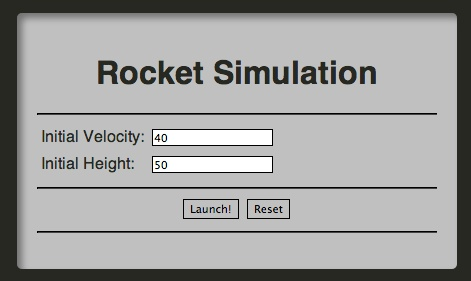
\includegraphics[width=1\textwidth]{Input.jpeg}\\
			\textit{Figure 2.1: A prototype of the input panel.}\\
		\end{centering}
			% \caption{Prototype of the input panel.}
		% \end{figure}
		It will present a data-representation of a flight based on the user's input and make this data accessible within the application and by download. \textit{See Figure 2.2}\\
		% \begin{figure}[h!]
		\begin{centering}
			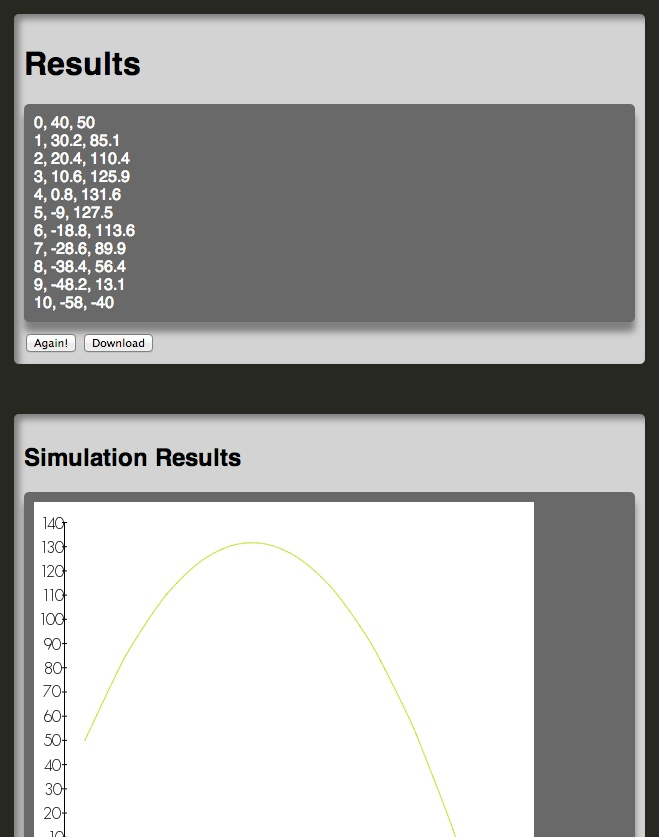
\includegraphics[width=.5\textwidth]{Output.jpeg}\\
			\textit{Figure 2.2: A prototype of the output panel.}\\
		\end{centering}
			% \caption{Prototype of the output.}
		% \end{figure}
		It will also present the user with a visual representation of the data in the form of line graphs.

		% \begin{itemize}
		% 	\item Present user with input interface
		% 	\item Present a data-representation of a flight based on the user's input
		% 	\item Make this data accessible by download
		% 	\item Present the user with a visual representation of the data (graph)
		% \end{itemize}
		% The target user is a student in a high school calculus class.

	\section{Constraints and Assumptions}
		\subsection{Constraints}
			The simulation will only represent one-dimensional motion.  It will take into account the height the rocket achieves, but will not consider any lateral distance.  It will run inside of a web browser, rather than being a native application. The application, being built in PHP, will require a web-server to run. PHP is a server-side language.
			% \begin{itemize}
			% 	\item Simulation is one-dimensional
			% 	\item Simulation is not a native application
			% \end{itemize}
		\subsection{Assumptions}
			The user must have an Internet-connected device or take it upon him/herself to host it locally.  It will require a web-server to run.  The application will most likely be nimble enough to run on a dial-up connection without incidence, but broadband connections are so common that we will build it with the assumption that the user has access to one and will not constrain ourselves to making it comfortable for a dial-up connection.
			% \begin{itemize}
			% 	\item User has a broadband Internet connection
			% \end{itemize}

	\section{Timeline}
		\begin{itemize}
			\item Simulation Guts.......................................September 25, 2012
			\item Basic Interface.......................................October 10, 2012
			\item Enter Alpha...........................................November 6, 2012
			\item Requirement Doc Draft.................................By January 31, 2013
			\item Spec Docs Finished....................................By February 14, 2013
			\item Graphs Implemented....................................By February 16, 2013
			\item Graphs Polished										By February 24, 2013\\
					\textit{Scaling, Hiding, etc.}
			\item Minor features implemented (Data validation, etc.)....By March 2, 2013
			\item Enter Beta............................................By March 4, 2013\\
					\textit{This phase will constitute user testing.}
			\item Ship..................................................By March 21, 2013
		\end{itemize}

\chapter{Requirements}
	\begin{itemize}
		\item Must produce accurate data\\
			\textit{Several sample data sets will be run by hand to ensure that the simulation is achieving this.}
		\item Export data as CSV via web interface
		\item Must produce graph of rocket's velocity height
			\begin{itemize}
				\item Graph must be properly labeled and scaled
				\item User must be able to view velocity and height both separately and together
				\\	  \textit{This will be done by check-boxes or radio buttons; client has no preference.}
			\end{itemize}
		\item Must work on any Internet connected device with a JavaScript-enabled, modern browser\\
				\textit{We define "Modern Browser" to mean released after 1/1/2011 and supporting HTML5 and CSS3.}
		\item Must list range of example input values for Initial Height and Initial Velocity\\
			\textit{As per client's request, input will be text boxes, rather than drop-down boxes.\\
					Data validation will be done, most likely, through JavaScript }
		\item System Portability will be ensured by the fact that the software is web-based and built in standard technologies (i.e., no plug-ins required).
	\end{itemize}
\chapter{Future Features}
	\begin{itemize}
		\item Client would like a loading screen with a graphic of a rocket flying in an arc.
	\end{itemize}
\end{document}